%----------------------------------------------------------------------------------------
%	3. Challenges of handling EHR data
%----------------------------------------------------------------------------------------

\subsection{Phenotyping}


\subsection{Evaluation}




\subsection{Knowledge Graph and Its Application}

With the rapid development of Internet technology, the storage and sharing of knowledge has become more and more convenient, followed by the exponential growth of the total amount of knowledge, knowledge in various fields is no longer an island, but in the ocean of the Internet mutual integration and cross-development. Since Google proposed "Knowledge Graph", this technology that can draw knowledge contexts, mine potential relationships between data, analyze semantic information, and visually provide users with knowledge information in the form of graphs has rapidly attracted research interests in various fields. At present, there have been many important research results, such as Dbpedia ~\cite{2007The} and so on. The predecessor of Knowledge Graph is the Semantic Web. The Semantic Web is dedicated to enabling computers to understand and process the semantic information expressed in texts, thereby supporting extensive and effective automatic reasoning in the network environment. As a knowledge carrier, the biggest advantage of knowledge graph is to visualize the return of knowledge, so that people can not only quickly sort out the logical context between professional knowledge, but also grasp the most critical knowledge points and quickly find the information they need.

\subsubsection{Composition of Knowledge Graph}

A knowledge graph consists of nodes and edges. The nodes in the knowledge graph represent concepts and entities, concepts are abstract things, and entities are concrete things; edges represent the relationships and attributes of things, the internal features of things are represented by attributes, and the external connections are represented by relationships. Many times, people simplify the description of the knowledge graph, refer to entities and concepts as entities, and relations and attributes as relationships, so that it can be said that knowledge graphs describe entities and the relationships between entities. Entities can be people, places, organizations, concepts, etc. There are more types of relationships, such as the relationship between people, the relationship between people and organizations, the relationship between concepts and an object, etc. is a six-tuple, which are entity 1, relation, entity 2, and constraints or properties for each element, expressed as {“entityl, entity1\_propority, relation, relation\_propority, entity2, entity2\_propority”}.

CMeKG uses Baidu's open source visualization library Echarts to display the knowledge graph. For each entity, select the six-tuple with the entity as the main subject to display, in which the three-tuple of the attribute description can be empty, that is, the six-tuple is in the attributes of both the entity and the relationship. When empty, it degenerates into a triple. As shown in ~\ref{fig:frog1}, nodes of the same color connected to the same node represent the same semantic relationship. The overall effect is a network structure centered on the query entity, and related entities with semantic relationships diverge to the surrounding, and the weight of each relationship edge equal.

\begin{figure}[ht]
\centering
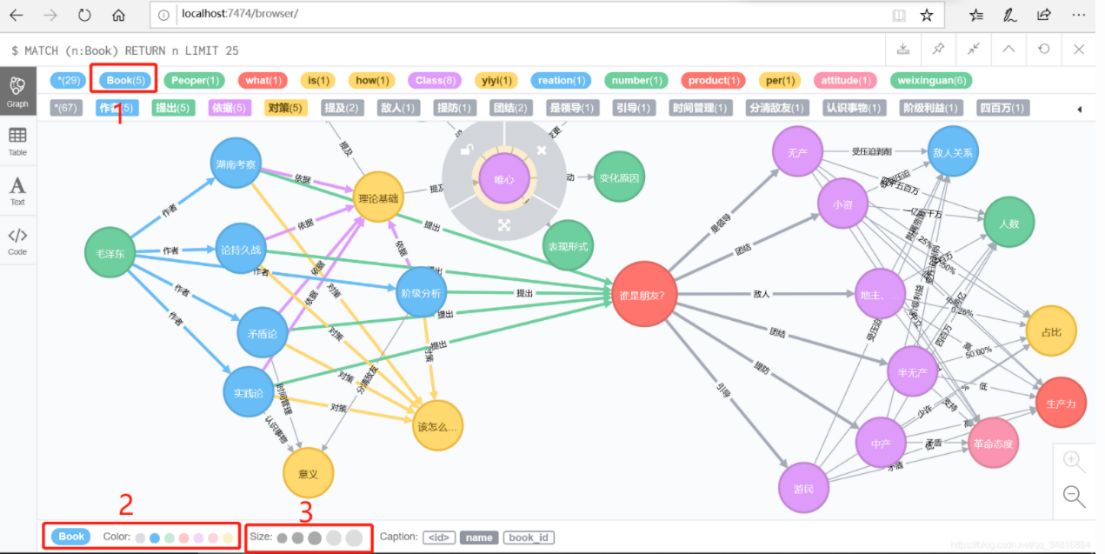
\includegraphics[width=1\textwidth]{images/3.3.1.png}
\caption{\label{fig:frog1}Knowledge graph visualization results}
\end{figure}

\subsubsection{ The construction process of knowledge graph}

The knowledge graph construction process includes four parts, namely data acquisition, information acquisition, knowledge fusion and knowledge processing. Among them, data acquisition is usually obtained through unstructured data (such as encyclopedic knowledge, papers, etc.), semi-structured data (such as HTML, various reports, etc.) and structured data (such as electronic medical records, etc.). Second, entity acquisition and triplet acquisition are the basis of the information acquisition stage, including named entity recognition~\cite{Kova2013Combining, 2013Recognizing}, triplet relation extraction~\cite{2017Learning} and relation attribute extraction. Entity recognition is to extract text entities according to relevant rules in a given knowledge text; relationship extraction refers to a series of discrete named entities obtained from a text corpus after entity extraction. Only by extracting the association relationship between entities and connecting the entities through the relationship can a networked knowledge structure be formed; attribute extraction is to extract other knowledge that may affect the relationship between entities. Knowledge fusion is to integrate the scattered information obtained in the process of "information acquisition". It is divided into two parts, entity linking and knowledge merging. Entity linking refers to connecting entity objects to the knowledge base. Among them, entity normalization~\cite{2017CNN, 2017A} is to unify the names of different nodes representing the same entity, so as to avoid the redundancy that may occur in the establishment stage of the knowledge graph; knowledge Merging mainly refers to data merging between different data sources, in order to further reduce the computing power consumed when establishing nodes and relationships. Finally, knowledge processing is the inspection and acceptance of the established knowledge graph function, including knowledge reasoning and quality assessment. Knowledge reasoning can assist decision-making through the method of graph embedding~\cite{2017Safe, 2019PrTransH}, thereby further expanding and enriching knowledge Network, quality assessment can quantify the credibility of knowledge, and ensure the quality of the knowledge base by discarding knowledge with low confidence.

\subsubsection{ Medical Knowledge Graph}

The construction of medical knowledge graph is mainly to extract entities, relationships and attributes from unstructured data manually or automatically. Since the research results of medical knowledge graph will help to promote the automation and intelligent processing of medical data, and have broad application prospects and social value, improving the construction of medical knowledge graph has become a current research hotspot. In the medical field, triples contain entities in multiple sub-fields such as genes, proteins, diseases, and drugs, and the data in each sub-field has the characteristics of strong specialization, unbalanced relationship distribution, and complex structure. At present, most medical knowledge graphs are constructed for a certain sub-field, such as Gene Ontology for genes, DrugBank for drugs, and UniProt for proteins, etc., all of which provide a better solution for the subsequent use of computational methods to solve inherent problems in this field. many possibilities. Building a domain-wide medical knowledge graph is more difficult and the knowledge sources are more complex, but it also has wider applicability. For example, Linked Life Data includes biomedical entities such as genes, proteins, drugs, and targets. Lin ~\cite{2020KGNN} et al. proposed the KGNN drug knowledge graph to predict the relationship between drugs, and researchers used a combination of multiple data sources to focus on the potential links between drugs; Wise ~\cite{2020COVID} et al. COVID-19 disease-specific knowledge map was proposed to accelerate information retrieval and discovery of scientific literature; in the same year, Li ~\cite{2020Automatic} et al. constructed a knee osteoarthritis disease-specific medical knowledge map based on the electronic medical records of knee osteoarthritis patients , and the specialized disease knowledge graph supports intelligent medical applications such as knowledge retrieval and decision support. The visualization results of the medical knowledge graph part are shown in Figure~\ref{fig:frog2}. Graphical visualization is an important part of the medical knowledge map. Various disease entities can be queried through the initial index or search box on the system page, and various entities and relationships related to the disease can be linked radioactively, which can effectively help Doctors and patients understand the disease knowledge and related diagnosis and treatment methods.

\begin{figure}[ht]
\centering
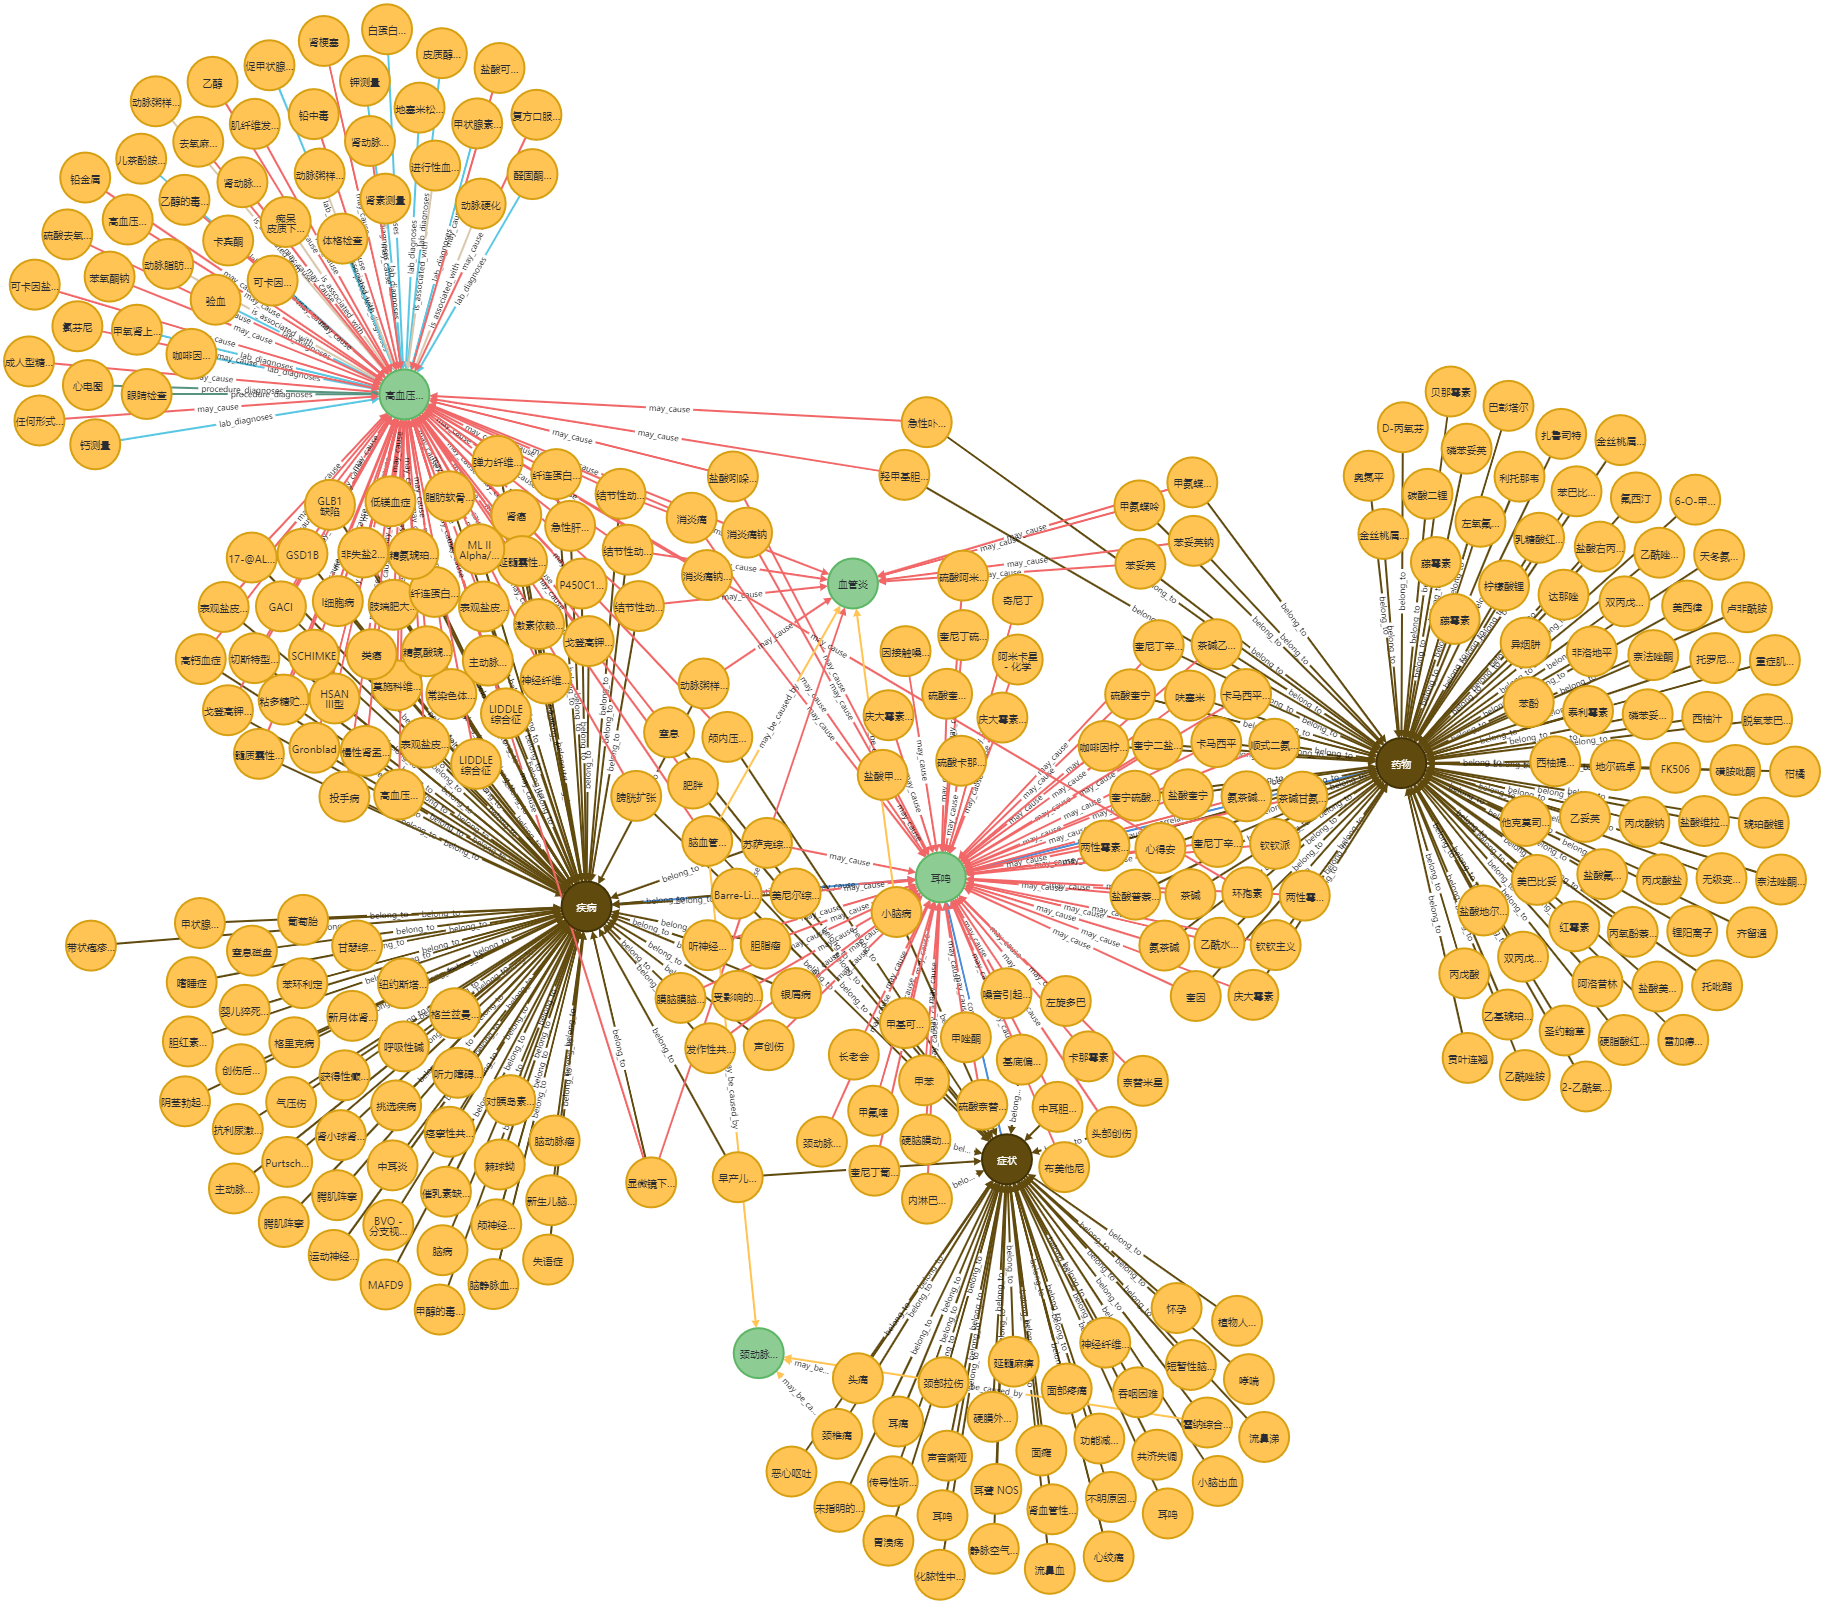
\includegraphics[width=1\textwidth]{images/3.3.2.png}
\caption{\label{fig:frog2}Partial visualization results of medical knowledge graph}
\end{figure}

\subsubsection{Application of Medical Knowledge Graph}

The application of knowledge graphs in the medical field helps to improve the level of medical intelligence. At present, medical knowledge graphs are mainly used in clinical decision support systems, medical intelligent semantic search engines, medical question answering systems, and medical knowledge popularization.

(1) Predict drug-target interactions. Although drug research has a long history, many discoveries of pharmacological effects are indeed accidental. Rarely is a drug linked to only one specific target, so it may be a better fit for another target, which enables drug repurposing. Traditional methods for finding unknown drug-target interactions (Drug-Target Interaction~\cite{Y2008Prediction}) include chemical genetic methods and proteomic methods. These traditional approaches are limited by their reliance on experimental manipulation and available resources, and can only handle a limited number of possible drugs and targets. The computational prediction method greatly improves the efficiency of the traditional method by virtue of the algorithm of graph structure and similarity measurement, but it is still limited by the algorithm itself and still has a high computational complexity.

As an alternative, TriModel ~\cite{2019Discovering} utilizes existing drug target knowledge graphs (such as DrugBank ~\cite{2017DrugBank} and KEGG ~\cite{2017KEGG}), treats drug target interaction prediction as a knowledge graph completion task, and constructs a knowledge graph embedding Semantic models to predict novel drug-target interactions. It is worth noting that TriModel also applies the relationship between other biological entities when training drug-target interactions, and the final predicted drug and target (gene) are in the middle, and the same way can also be used to predict other entities. relationship, such as the association between proteins. In addition, Liang et al. ~\cite{2019Predicting} also used the knowledge graph embedding method to predict new drug-target interactions. The model integrates the translation model and the graph embedding, which solves the problem that the translation model does not perform well in some unbalanced relationships.

(2) Build a clinical decision support system. The key to enabling precision medicine is a clinical decision support system, like a question-and-answer system that receives questions from clinicians and patients and returns clinical answers. An efficient clinical decision support system can not only reduce the pressure on clinicians, but also enable accurate diagnosis of diseases and personalized and precise treatment for patients. Such efficiency mainly benefits from the electronic medical record system and medical knowledge graph behind it, on which many clinical decision support systems are built. With the help of the medical knowledge graph, the clinical diagnosis decision support system can provide intelligent diagnosis, treatment plan recommendation and referral guide based on patient symptom description and laboratory data, and can also analyze and fill in gaps in the doctor's diagnosis and treatment plan to reduce or even avoid misdiagnosis .

For example, Goodwm et al. ~\cite{2016Medical} constructed a disease-specific knowledge graph based on the accumulated electronic medical record data, and then used this knowledge graph to reason about the received questions to obtain a candidate answer set, and finally sorted and selected the relevant medical literature to obtain a set of candidate answers. Improve the quality of answers. In addition, Zhao et al. ~\cite{2018EMR} constructed a medical knowledge network composed of medical entities and medical relations, regarded the network as a Markov random field, and performed probabilistic reasoning according to the knowledge graph embedding method. More systematically, Sheng~\cite{2018A} et al. constructed a clinical decision support platform dual-driven by medical sample database and medical knowledge graph, which can provide a series of clinical decision support services such as query, diagnosis, examination, treatment and prognosis.

(3) Radiology report generation driven by medical knowledge graph. Zhang et al.~\citet{2020When} established a map of 20 diseases in the chest through prior knowledge, and established links between 20 related diseases, where diseases were defined as nodes, and then embedded the graph model into the backbone network, as shown in Figure~\ref{fig:frog3} shown.

\begin{figure}[ht]
\centering
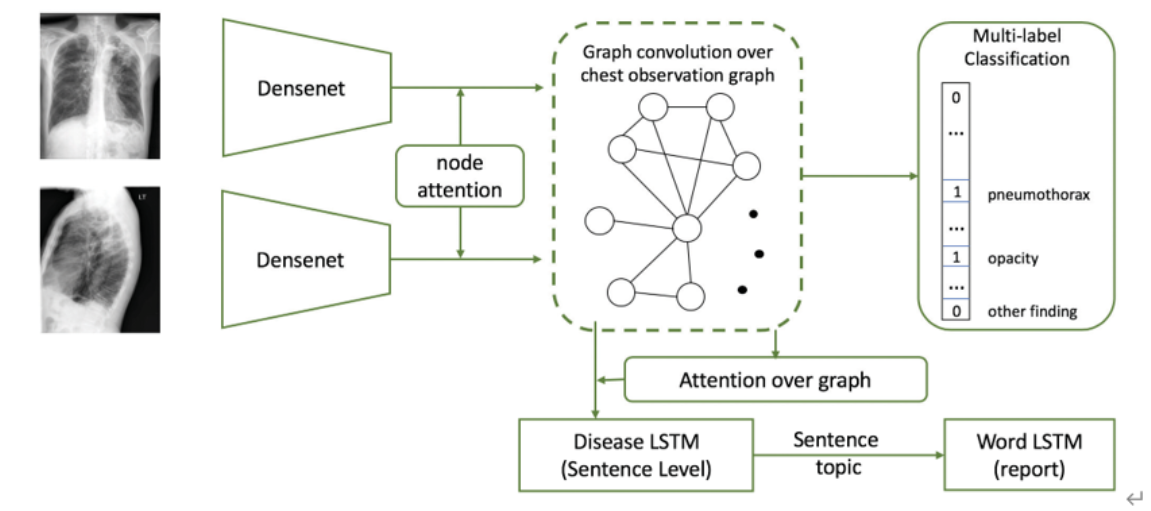
\includegraphics[width=1\textwidth]{images/3.3.3.png}
\caption{\label{fig:frog3}Framework of radiology report generation integrated with knowledge graph}
\end{figure}


The knowledge is combined with the image information generated by the Densenet neural network to train a multi-class label network, where each class corresponds to a node. A topic-level and sentence-level LSTM network is simultaneously trained to compose the decoder to generate reports.




\subsection{Feature selection} % 3.4

\subsubsection{Importance}
Feature selection is to extract valuable information from noisy or large-scale medical data. Specifically, researchers would rule out redundant or irrelevant features in data preprocessing. 

For example, available information for disease diagnosis could be various features, ranging from basic data(weight, age, gender, etc.) to complicated CUI data extracted from unstructured medical notes. Some could be potentially effective for the task while others are just noises. In this case, it is necessary to consider how to carry out feature selection carefully. 

\subsubsection{Some common methods}
\xhdr{Univariate analysis} It is easy and convenient to implement some traditional statistical methods for feature selection, such as Correlation Coefficient Method, Mutual Information method and Chi-square Test.

\xhdr{Lasso regression} Lasso, namely L1 Regularization, is a modification of linear regression. By constructing an L1 penalty in the loss function, the coefficients of some features can be compressed and changed to 0, so as to achieve the purpose of feature selection. 

\xhdr{Decision tree algorithm} Random Forest is a commonly used decision tree algorithm, with the ability to measure the feature importance. As a kind of ensemble learning, Random Forest is based on the bootstrap aggregation (bagging) of decision trees.


\subsection{Unbalanced data sampling} % 3.5


\subsection{Missing values imputation} % 3.6
In datasets, we often call the variables without missing values as complete variables, and the variables with missing values as incomplete variables. Here are some different types of missing data:
\subsubsection{Type of missing values}
\begin{itemize}
\item \textbf{Missing at random, MAR.}
Random loss means that the probability of data loss has nothing to do with the lost data itself, but only with some observed data. In other words, the lack of data is not completely random, and the lack of such data depends on other complete variables. For example, men only get testicular cancer, and the data of women suffering from testicular cancer is empty. If drug a and drug B have adverse reactions, the drug B characteristics of patients using drug a are usually empty. When screening patients, if female patients or patients who only use drug a are not taken as the research criteria, the characteristics of whether they have testicular cancer, whether they use drug a and whether they use drug B will appear in the data set.

\item \textbf{Missing completely at random, MCAR.}
The lack of data is completely random, does not depend on any incomplete variables or complete variables, and does not affect the unbiased nature of the sample. Simply put, the probability of data loss is completely independent of its assumed value and other variable values. It is most likely to occur in the absence caused by human error.

\item \textbf{Missing not at random, MNAR.}
The lack of data is related to the value of incomplete variables themselves. There are two situations: the missing value depends on its hypothetical value (for example, high-income people usually do not want to disclose their income in the survey); Alternatively, the missing value depends on the value of other variables (assuming that women usually don't want to disclose their age, here the missing value of age variable is affected by gender variable).

In the first two cases, the missing value data can be deleted according to its occurrence. At the same time, the random missing value can be estimated by known variables. In the third case, deleting data containing missing values may lead to deviation of the model, and special care should be taken to fill in the data. At present, there is no set of standard criteria for determining the type of missing value. Most judgments are based on experience or business.
\end{itemize}

\subsubsection{Causes of missing values}
\begin{enumerate}

\item Information is temporarily unavailable. For example, the income of a product has a lag effect.

\item Data is not recorded, omitted or lost due to human factors, which is the main reason for data loss.

\item Data loss caused by failure of data acquisition equipment, storage medium and transmission medium.

\item The cost of obtaining this information is too high.

\item One or some attributes of some objects are unavailable; Such as: unmarried spouse's name, children's fixed income status, etc.

\item The real-time performance requirements of the system are high, that is, it is required to make judgments or decisions quickly before obtaining these information.
\end{enumerate}

\subsubsection{What are the effects of missing values in data analysis}
\begin{itemize}
\item Make the system lose a lot of useful information
\item It makes the uncertainty in the system more obvious, and it is more difficult to grasp the deterministic components contained in the system
\item Data containing null values will make the data mining process into chaos and lead to unreliable output
\end{itemize}
\subsubsection{Missing value processing method}
\begin{itemize}
\item \textbf{Delete}
\item \textbf{Interpolation}
\begin{itemize}
\item Manual
\item Default
\item Based on statistics
\end{itemize}
\item \textbf{Based on Clustering}
\begin{itemize}
\item Single neighbor
\item K neighbors
\end{itemize}
\item \textbf{Regression}

When the variable is not linearly correlated, it will lead to biased estimation

\item \textbf{Expectation maximization (EM)}

\item \textbf{Multiple imputation (MI)}

\item \textbf{Agency features}

Fill in missing values by looking for the relationship between attributes. It looks for two attributes with the greatest correlation between them. One without missing value is called proxy attribute and the other is called original attribute. Proxy attribute is used to determine the missing value in the original attribute

\item \textbf{Do not process missing values}

A method of data mining directly on data containing null values. These include: Bayesian network and artificial neural network. Bayesian network provides a natural method to represent the causal information between variables, which is used to find the potential relationship between data. In this network, nodes are used to represent variables, and directed edges are used to represent the dependencies between variables. Bayesian network is only suitable for those who have a certain understanding of domain knowledge, at least when the dependence between variables is clear. Otherwise, learning the structure of Bayesian network directly from the data not only has high complexity (with the increase of variables, the exponential level increases), the cost of network maintenance is expensive, but also has many estimation parameters, which brings high square error to the system and affects its prediction accuracy.

\end{itemize}


\subsection{Dimensionality reduction} % 3.6
\subsubsection{Importance}
Selected features would be mapped to the corresponding feature vectors, which are to be fed into the model later. However, due to the constraints of computing resources, researchers would take dimensionality reduction into consideration. Specifically, they would convert high dimensional vectors to low dimensional vectors for a better use.

\subsubsection{Common methods}
\xhdr{PCA} PCA(Principal Component Analysis) is an unsupervised algorithm for dimensionality reduction. After some matrix transformation steps based on data distribution, PCA would extract the principal features of the data.

\xhdr{AutoEncoder} AutoEncoder, as a part of the encoder-decoder structure, is trained based on the reconstruction error. The middle layer of the encoder-decoder architecture could capture the principal features of the original data through the end-to-end learning process.

\subsection{Difference of EMRs describe habit}%3.8书写习惯问题 ziwei
Many hospitals now have outlines and templates in order to standardize electronic medical record documents. Therefore, when writing a case, it is not necessary for the doctor to write word by word, and there is a corresponding template to choose from. The same hospital should have the same structure. But putting together EMR samples from different hospitals makes a difference. The descriptions are different and the ratings are different.\\
\\For example, some hospitals describe the situation of consciousness only as coma. But there are also three similar but different states, like syncope and shock.
\\Coma has three stages, mild, moderate, and deep.
In such a situation, during preprocessing, several representations should be counted first, and finally these degrees should be sorted according to clinical prior knowledge and then quantified.

\xhdr{The natural language of EMRs also needs normalization}

The task of clinical term standardization is an indispensable task in medical statistics. Clinically, there are often hundreds of different ways of writing about the same diagnosis, operation, medicine, examination, test, symptom, etc.

The problem to be solved by standardization (normalization) is to find corresponding standard statements for various clinical statements.

With the basis of terminology standardization, researchers can conduct subsequent statistical analysis of electronic medical records. Essentially, the clinical term standardization task is also a kind of semantic similarity matching task.

However, because the expressions of the original words are too diverse (and the sentences are too short and the amount of information is too small), it is difficult for a single matching model to achieve good results.













